\section{Methodology}

\begin{frame}{Phase 1.1 - Literature Review}

    A deep literature review to \textbf{better understand the state of the art in Ammonia combustion and the challenges associated with it} will be conducted.
    We will focus on the following topics:

    \begin{itemize}
        \item Combustion dynamics in ICE\footnotemark[1] (flow engineering).
        \item Combustion modeling and CFD\footnotemark[2] simulation for traditional fuels.
        \item Advanced and \textbf{optimized algorithms for numerical simulation of a two-phase dispersed turbulent flow}.
        \item Pollution and emissions from Ammonia derivate combustion products.
    \end{itemize}

    For our research, we will use \texttt{ScienceDirect}, \texttt{Scopus}, \texttt{IEEE Xplore} as main databases.

    A non-exhaustive list of applicable keywords: \textit{Ammonia, Combustion, two-phase dispersed turbulent flow, flash-boiling condition, ICE, CFD}.

    \footnotetext[1]{ICE: Internal Combustion Engine}
    \footnotetext[2]{CFD: Computational Fluid Dynamics}

\end{frame}



\begin{frame}{Phase 1.2 - Model Development}

    An \textbf{accurate and reliable model for Ammonia dynamics (non-reactive)} will be developed starting from previous knowledge of the literature review and experimental data founds.

    From a first analysis of the physics of the problem, we can expect our CFD model to be based on:

    \begin{itemize}
        \item An \textbf{Eulerian algorithm} dedicated to \textbf{advance in time the flow fields} by solving the Low-Mach number formulations of the Navier-Stokes equations
        \item A \textbf{Lagrangian solver} designed to synchronously \textbf{evolve the mass, momentum, and temperature equations} of dispersed droplets under point-particle approximation.
    \end{itemize}

    The model will be developed in \texttt{OpenFOAM} and \texttt{Chemkin}.

\end{frame}



\begin{frame}{Phase 1.3 - Model Validation}

    The model will be \textbf{validated using experimental data} from the literature.

    \vspace{9pt}

    \begin{columns}[c, onlytextwidth]

        \begin{column}{0.5\textwidth}

            \begin{figure}
                \centering

                \resizebox{0.8\columnwidth}{!}{%
                    \begin{tikzpicture}[node distance=1.5cm]

                        \node (development) [process] {Model Development};
                        \node (decision) [decision, below of=development, yshift=-0.5cm] {Valid?};

                        \node (analysis) [process, right of=decision, xshift=1.5cm] {Data Analysis};
                        \node (experiments) [process, below of=decision, yshift=-0.5cm] {Next Phase};

                        \draw [arrow] (development) -- (decision);
                        \draw [arrow] (decision) -- node[anchor=east] {Yes} (experiments);
                        \draw [arrow] (decision) -- node[anchor=south] {No} (analysis);
                        \draw [arrow] (analysis) |- (development);

                    \end{tikzpicture}
                }

            \end{figure}

        \end{column}

        \begin{column}{0.5\textwidth}

            Evaluation test cases are dependent on the literature review and the experimental data founds.

            If available, the following metrics will be adopted:

            \begin{itemize}
                \item Droplet size distribution.
                \item Temperature and pressure profiles.
                \item Spray geometry (angle, penetration, and shape).
            \end{itemize}

        \end{column}

    \end{columns}

\end{frame}



\begin{frame}{Phase 2.1 - Experimental Campaign}

    In the optic of gathering as many data as possible, an \textbf{experimental campaign with some preexisting injector in the context of Ammonia combustion in ICE} will be conducted.

    \vspace{9pt}

    \begin{columns}[c, onlytextwidth]

        \begin{column}{0.6\textwidth}

            Main goal: better understand the combustion process of Ammonia in an ICE (\textbf{reactive environment}).

            \vspace{9pt}

            Possible instruments to be used:

            \begin{itemize}
                \item High-speed camera.
                \item Pressure and temperature sensors.
                \item Gas analyzer.
            \end{itemize}

        \end{column}

        \begin{column}{0.4\textwidth}

            \begin{figure}
                \centering
                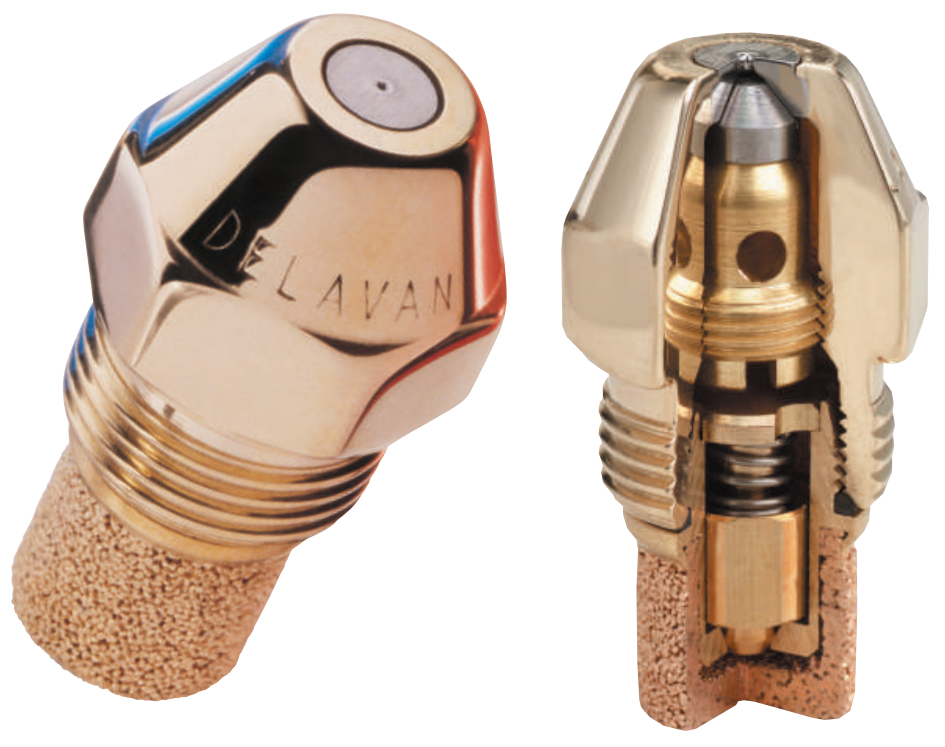
\includegraphics[width=0.9\columnwidth]{img/Delavan-nozzle.png}
                \caption{\texttt{Delavan} hollow cone nozzle that may be adopted.}
            \end{figure}

        \end{column}

    \end{columns}

\end{frame}



\begin{frame}{Phase 2.2 - Data Analysis}

    \begin{columns}[c, onlytextwidth]

        \begin{column}{0.5\textwidth}

            \begin{figure}
                \centering

                \resizebox{0.7\columnwidth}{!}{%
                    \begin{tikzpicture}[node distance=1.5cm]

                        \node (experiments) [io] {Experimental Campaign Data};
                        \node (analysis) [process, below of=experiments] {Data Analysis};
                        \node (correction) [process, below of=analysis] {Model correction};
                        \node (decision) [decision, below of=correction, yshift=-0.5cm] {Fitting?};
                        \node (design) [process, below of=decision, yshift=-0.5cm] {Next Phase};

                        \draw [arrow] (experiments) -- (analysis);
                        \draw [arrow] (analysis) -- (correction);
                        \draw [arrow] (correction) -- (decision);
                        \draw [arrow] (decision) -- node[anchor=east] {Yes} (design);
                        \draw [arrow] (decision.east) -- node[auto] {No} ++(20pt,0pt) |- (correction.east);

                    \end{tikzpicture}
                }

            \end{figure}

        \end{column}

        \begin{column}{0.5\textwidth}

            For each experimental test, data will be collected and analyzed.

            \vspace{9pt}

            The following analysis methods might be exploited:

            \begin{itemize}
                \item Data visualization.
                \item Machine learning.
                \item Statistical analysis.
            \end{itemize}

        \end{column}

    \end{columns}

\end{frame}



\begin{frame}{Phase 3 - Fuel Injector Design \& Testing}

    After the final model validation, the \textbf{design of the new injector} will follow.

    \vspace{9pt}

    \begin{columns}[c, onlytextwidth]

        \begin{column}{0.5\textwidth}

            As the CAD system, \texttt{CATIA V5} will be used.

            \vspace{9pt}

            The key factors driving our design will be:

            \begin{itemize}
                \item Stable flame inside the combustion chamber
                \item Low-to-zero $\mathrm{NO_x}$ emissions
            \end{itemize}

        \end{column}

        \begin{column}{0.5\textwidth}

            \begin{figure}
                \centering
                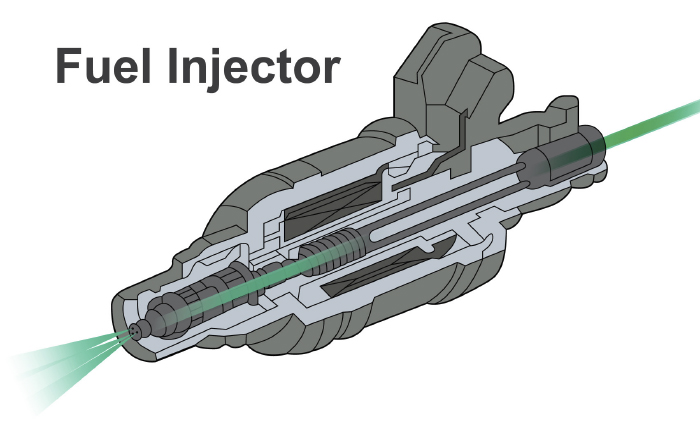
\includegraphics[width=0.9\columnwidth]{img/Fuel-injector.jpg}
            \end{figure}

        \end{column}

    \end{columns}

    \vspace{9pt}

    The new design will be \textbf{tested in a real ICE} and the data collected will be used \textbf{to evaluate its performance}.

\end{frame}